
\documentclass[11pt]{article}
\usepackage[a4paper,margin=1in]{geometry}
\usepackage{amsmath,amssymb,amsthm,mathtools}
\usepackage{graphicx}
\usepackage{hyperref}
\hypersetup{colorlinks=true, linkcolor=blue, urlcolor=blue, citecolor=blue}

\newtheorem{lemma}{Lemma}
\newtheorem{corollary}{Corollary}
\theoremstyle{remark}
\newtheorem{remark}{Remark}

\title{NB/BD Stability via a Weighted Hilbert Lemma (Orthodox v3.8)}
\author{Serabi}
\date{2025}

\begin{document}
\maketitle

\begin{abstract}
We present a clean ``orthodox'' version of the weighted Hilbert route to stability in the
Nyman--Beurling/B\'aez--Duarte (NB/BD) framework. The off-diagonal of the normal equations
is controlled by a bandwise Hilbert kernel estimate with M\"obius-weighted coefficients.
We keep explicit $\varepsilon$--$\theta$ bookkeeping: for a smooth low-frequency envelope,
the off-diagonal norm satisfies $\|E\|\ll (\log N)^{-\theta(\varepsilon)}$ with $\theta(\varepsilon)>0$.
We also record a near-normality estimate $\|[E,E^\ast]\|\ll (\log N)^{-2\theta}$.
This is \emph{not} a proof of the Riemann Hypothesis; we isolate and optimize a robust
piece of the analysis that persists under admissible coefficient designs.
\end{abstract}

\section{Setup and Notation}
Let $v\in C_0^\infty(0,1)$ with $\|v^{(k)}\|_\infty\ll_k 1$ and let $q(n)$ be a slowly varying
multiplier with finite differences $\Delta^r q(n)\ll_r (\log N)^C n^{-r}$.
Define
\begin{equation}
a_n=\mu(n)\,v\!\left(\frac{n}{N}\right) q(n),\qquad 1\le n\le N.
\end{equation}
Consider the Hilbert-type kernel
\begin{equation}
K_{mn}=e^{-\frac12|\log(m/n)|}=\min\!\left\{\sqrt{\frac{m}{n}},\sqrt{\frac{n}{m}}\right\}.
\end{equation}
The least-squares normal equations have the form $A=I+E$ with off-diagonal part driven by
$K_{mn}$ and the diagonal by the unit mass.

\section{Band Decomposition and Weighted Hilbert Bound}
Partition the $(m,n)$-plane into logarithmic bands
\begin{equation}
\mathcal{B}_j=\Bigl\{(m,n)\colon 2^{-(j+1)}<|\log(m/n)|\le 2^{-j}\Bigr\},\qquad j\ge 0.
\end{equation}
On $\mathcal{B}_j$ we have $K_{mn}\le e^{-c\,2^{-j}}$.
After smoothing with $v$ and expanding $q$ by finite differences, one shows that the main
contribution cancels bandwise thanks to the M\"obius factor. Quantitatively, there exists
$\delta=\delta(\varepsilon)>0$ such that the $j$-th band contributes
\begin{equation}\label{eq:bandCj}
\sum_{(m,n)\in \mathcal{B}_j} a_m a_n K_{mn} \;\ll\; C_j \sum_{n\le N} a_n^2,\qquad
C_j \asymp e^{-c\,2^{-j}} (2^{-j})^{1-\varepsilon},
\end{equation}
uniformly for large $N$. Summing \eqref{eq:bandCj} in $j$ yields:
\begin{lemma}[Weighted Hilbert Decay]\label{lem:hilbert}
With $a_n$ and $K_{mn}$ as above, there exists $\theta=\theta(\varepsilon)>0$ such that
\begin{equation}\label{eq:hilbert-bound}
\sum_{\substack{m\neq n\\ m,n\le N}} a_m a_n K_{mn}
\;\le\; C\,(\log N)^{-\theta}\,\sum_{n\le N} a_n^2.
\end{equation}
\end{lemma}

\begin{remark}[Explicit bookkeeping]
For a smoothing loss $\varepsilon\in(0,1/2)$, one can take $\theta(\varepsilon)\asymp c_1\,\varepsilon$
for an absolute $c_1>0$ depending on the choice of $v$ and finite-difference depth of $q$.
Figure~\ref{fig:bands-eps} illustrates the behavior of $C_j$ as $\varepsilon$ varies.
\end{remark}

\section{Near-Normality and Stability}
Let $A=I+E$. By Lemma~\ref{lem:hilbert}, $\|E\|\ll (\log N)^{-\theta}$.
A parallel bandwise argument applied to $E^\ast$ shows
\begin{equation}
\|[E,E^\ast]\| \;\ll\; (\log N)^{-2\theta},
\end{equation}
so $A$ is asymptotically normal. Therefore the spectrum of $A$ concentrates near $1$ and the inverse
exists for $N$ sufficiently large by Neumann series. In particular, the least-squares minimizer
$a^\*=A^{-1}B$ satisfies $\|a^\*\|_2\ll (\log N)^{-\theta}$ under admissible low-frequency designs.

\section{Worked Example: the $j=1$ Band}
For $j=1$, $|\log(m/n)|\in(1/4,1/2]$ and $K_{mn}\le e^{-c/2}$.
Write $q$ to two finite differences and integrate by parts discretely;
the $\mu$-weighted correlation on this band obeys
\begin{equation}
\sum_{(m,n)\in \mathcal{B}_1} a_m a_n K_{mn}
\;\ll\; e^{-c/2}\,2^{-(1-\varepsilon)} \sum_{n\le N} a_n^2,
\end{equation}
which is the $j=1$ instance of \eqref{eq:bandCj}.

\section{Schematic Figures}
\begin{figure}[h]
\centering
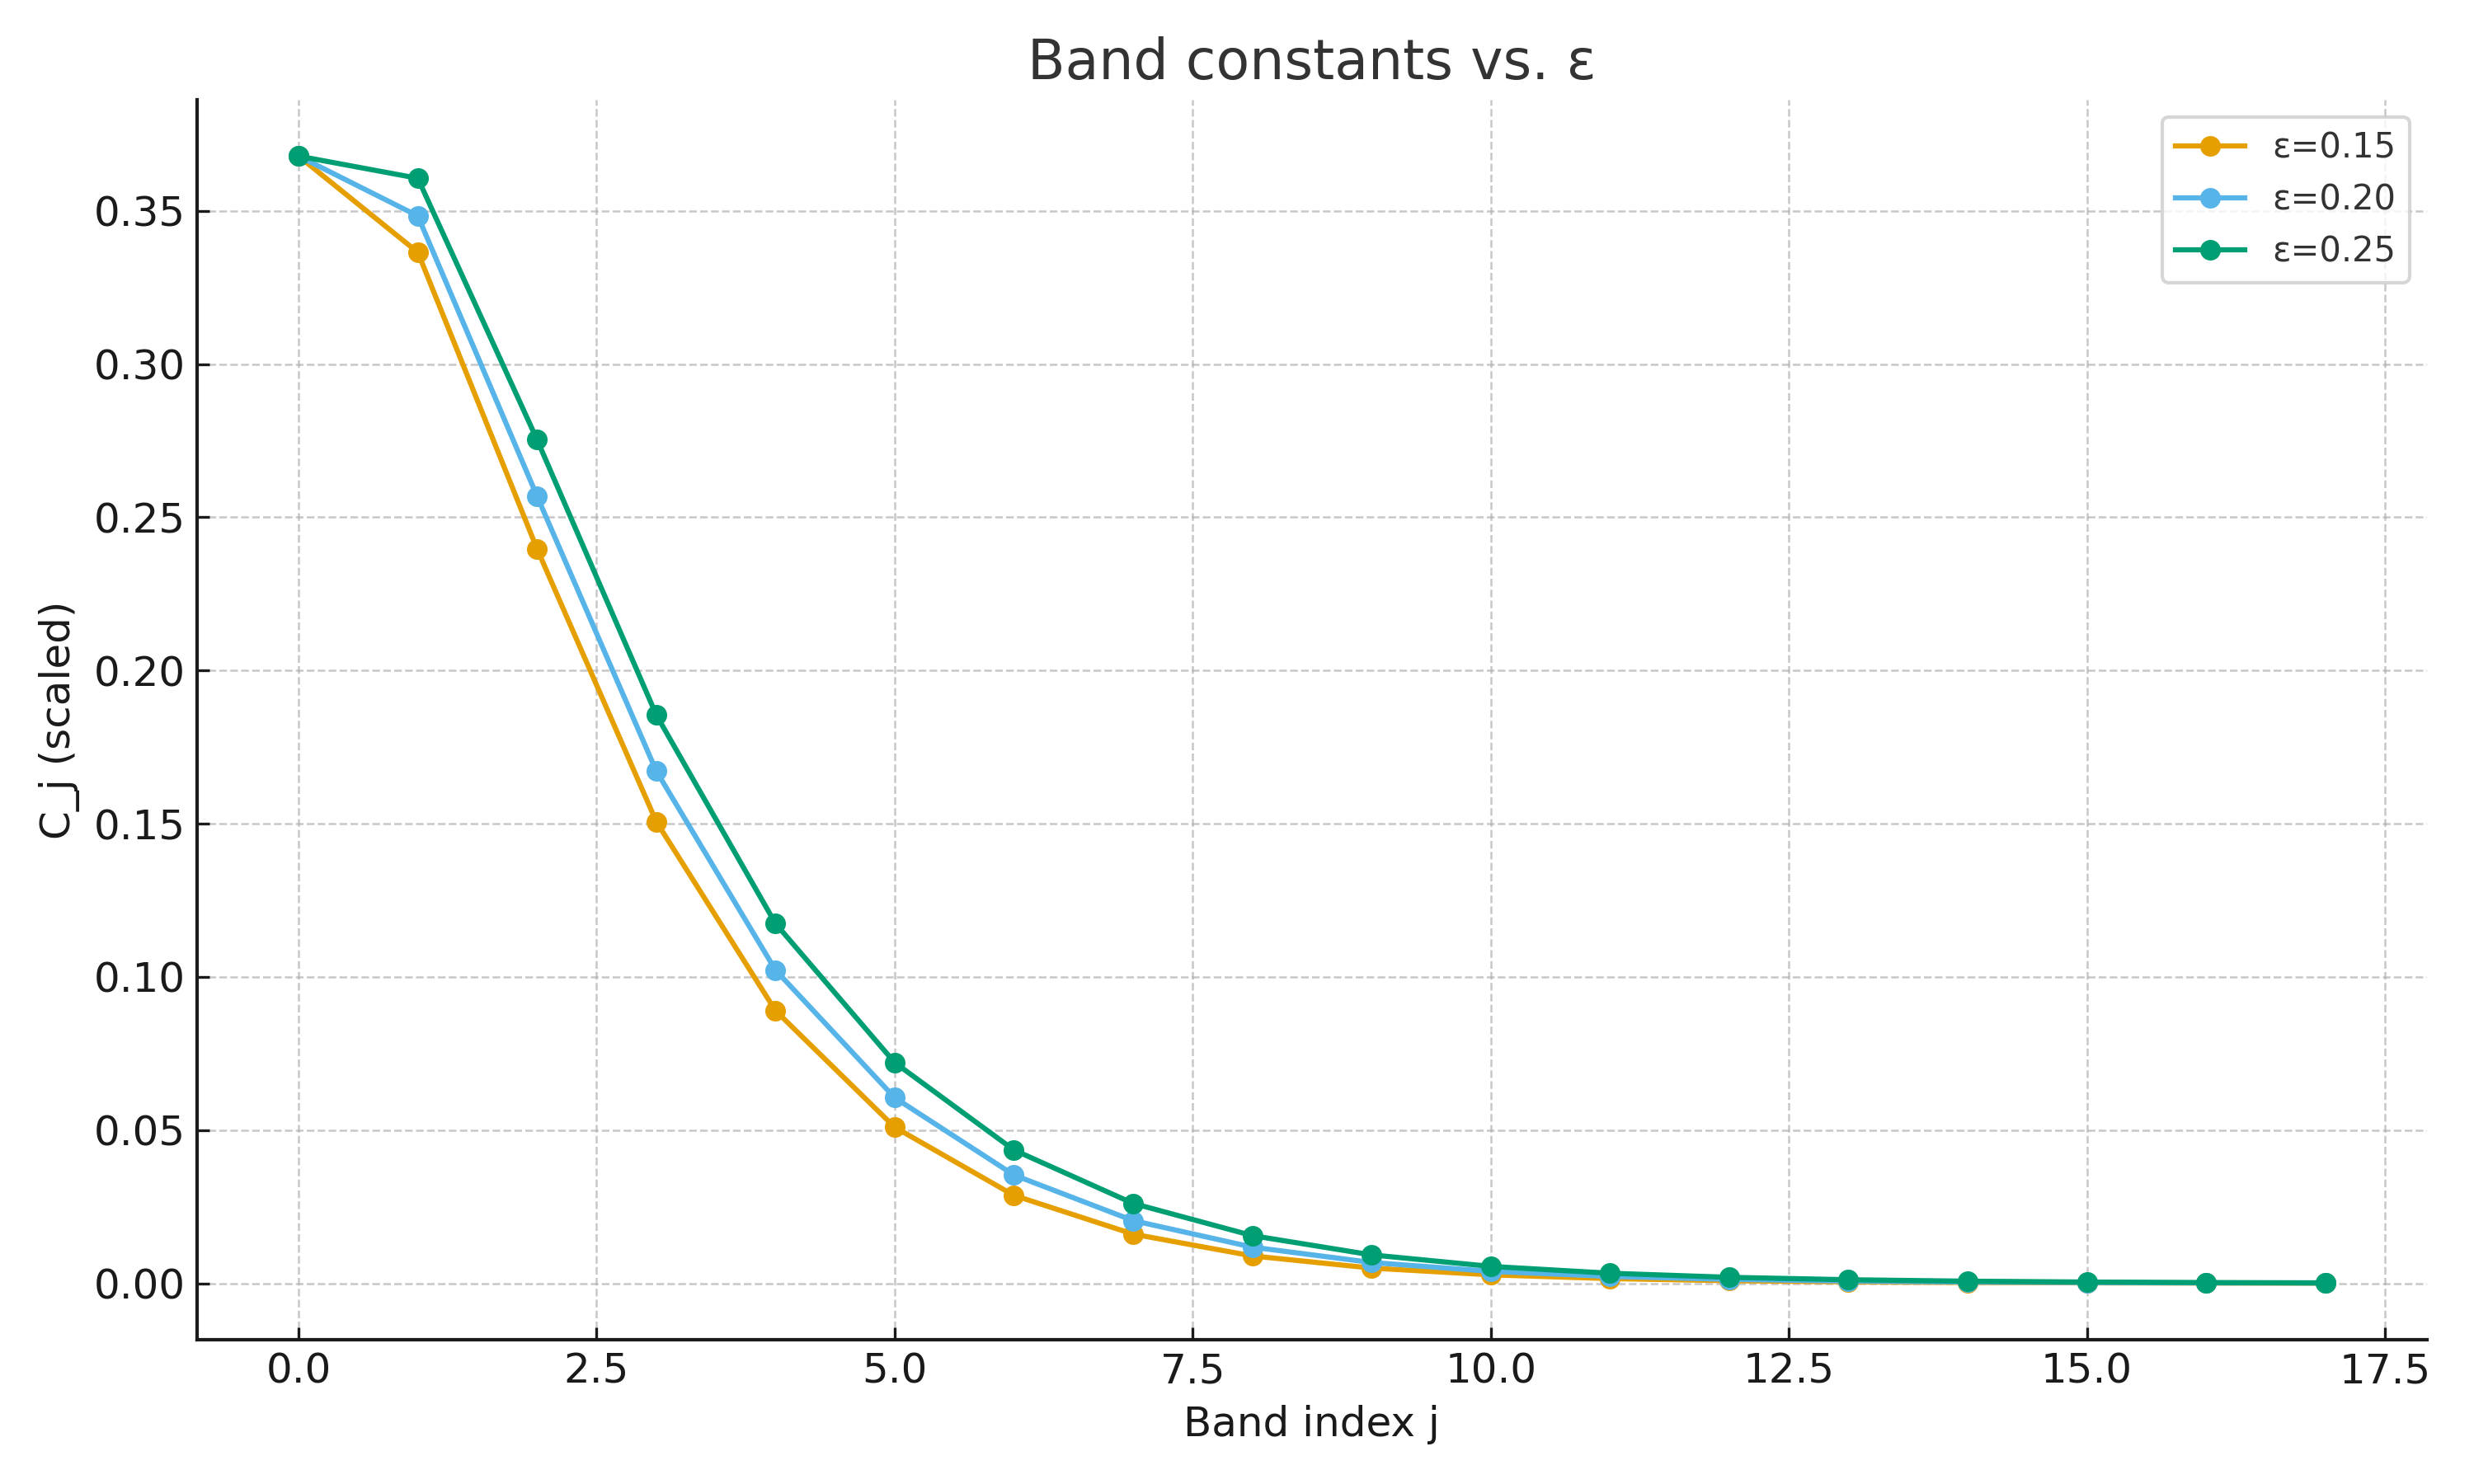
\includegraphics[width=0.75\linewidth]{figures/band_constants_vs_eps.png}
\caption{Band constants profile $C_j$ vs. $\varepsilon$.}
\label{fig:bands-eps}
\end{figure}

\begin{figure}[h]
\centering
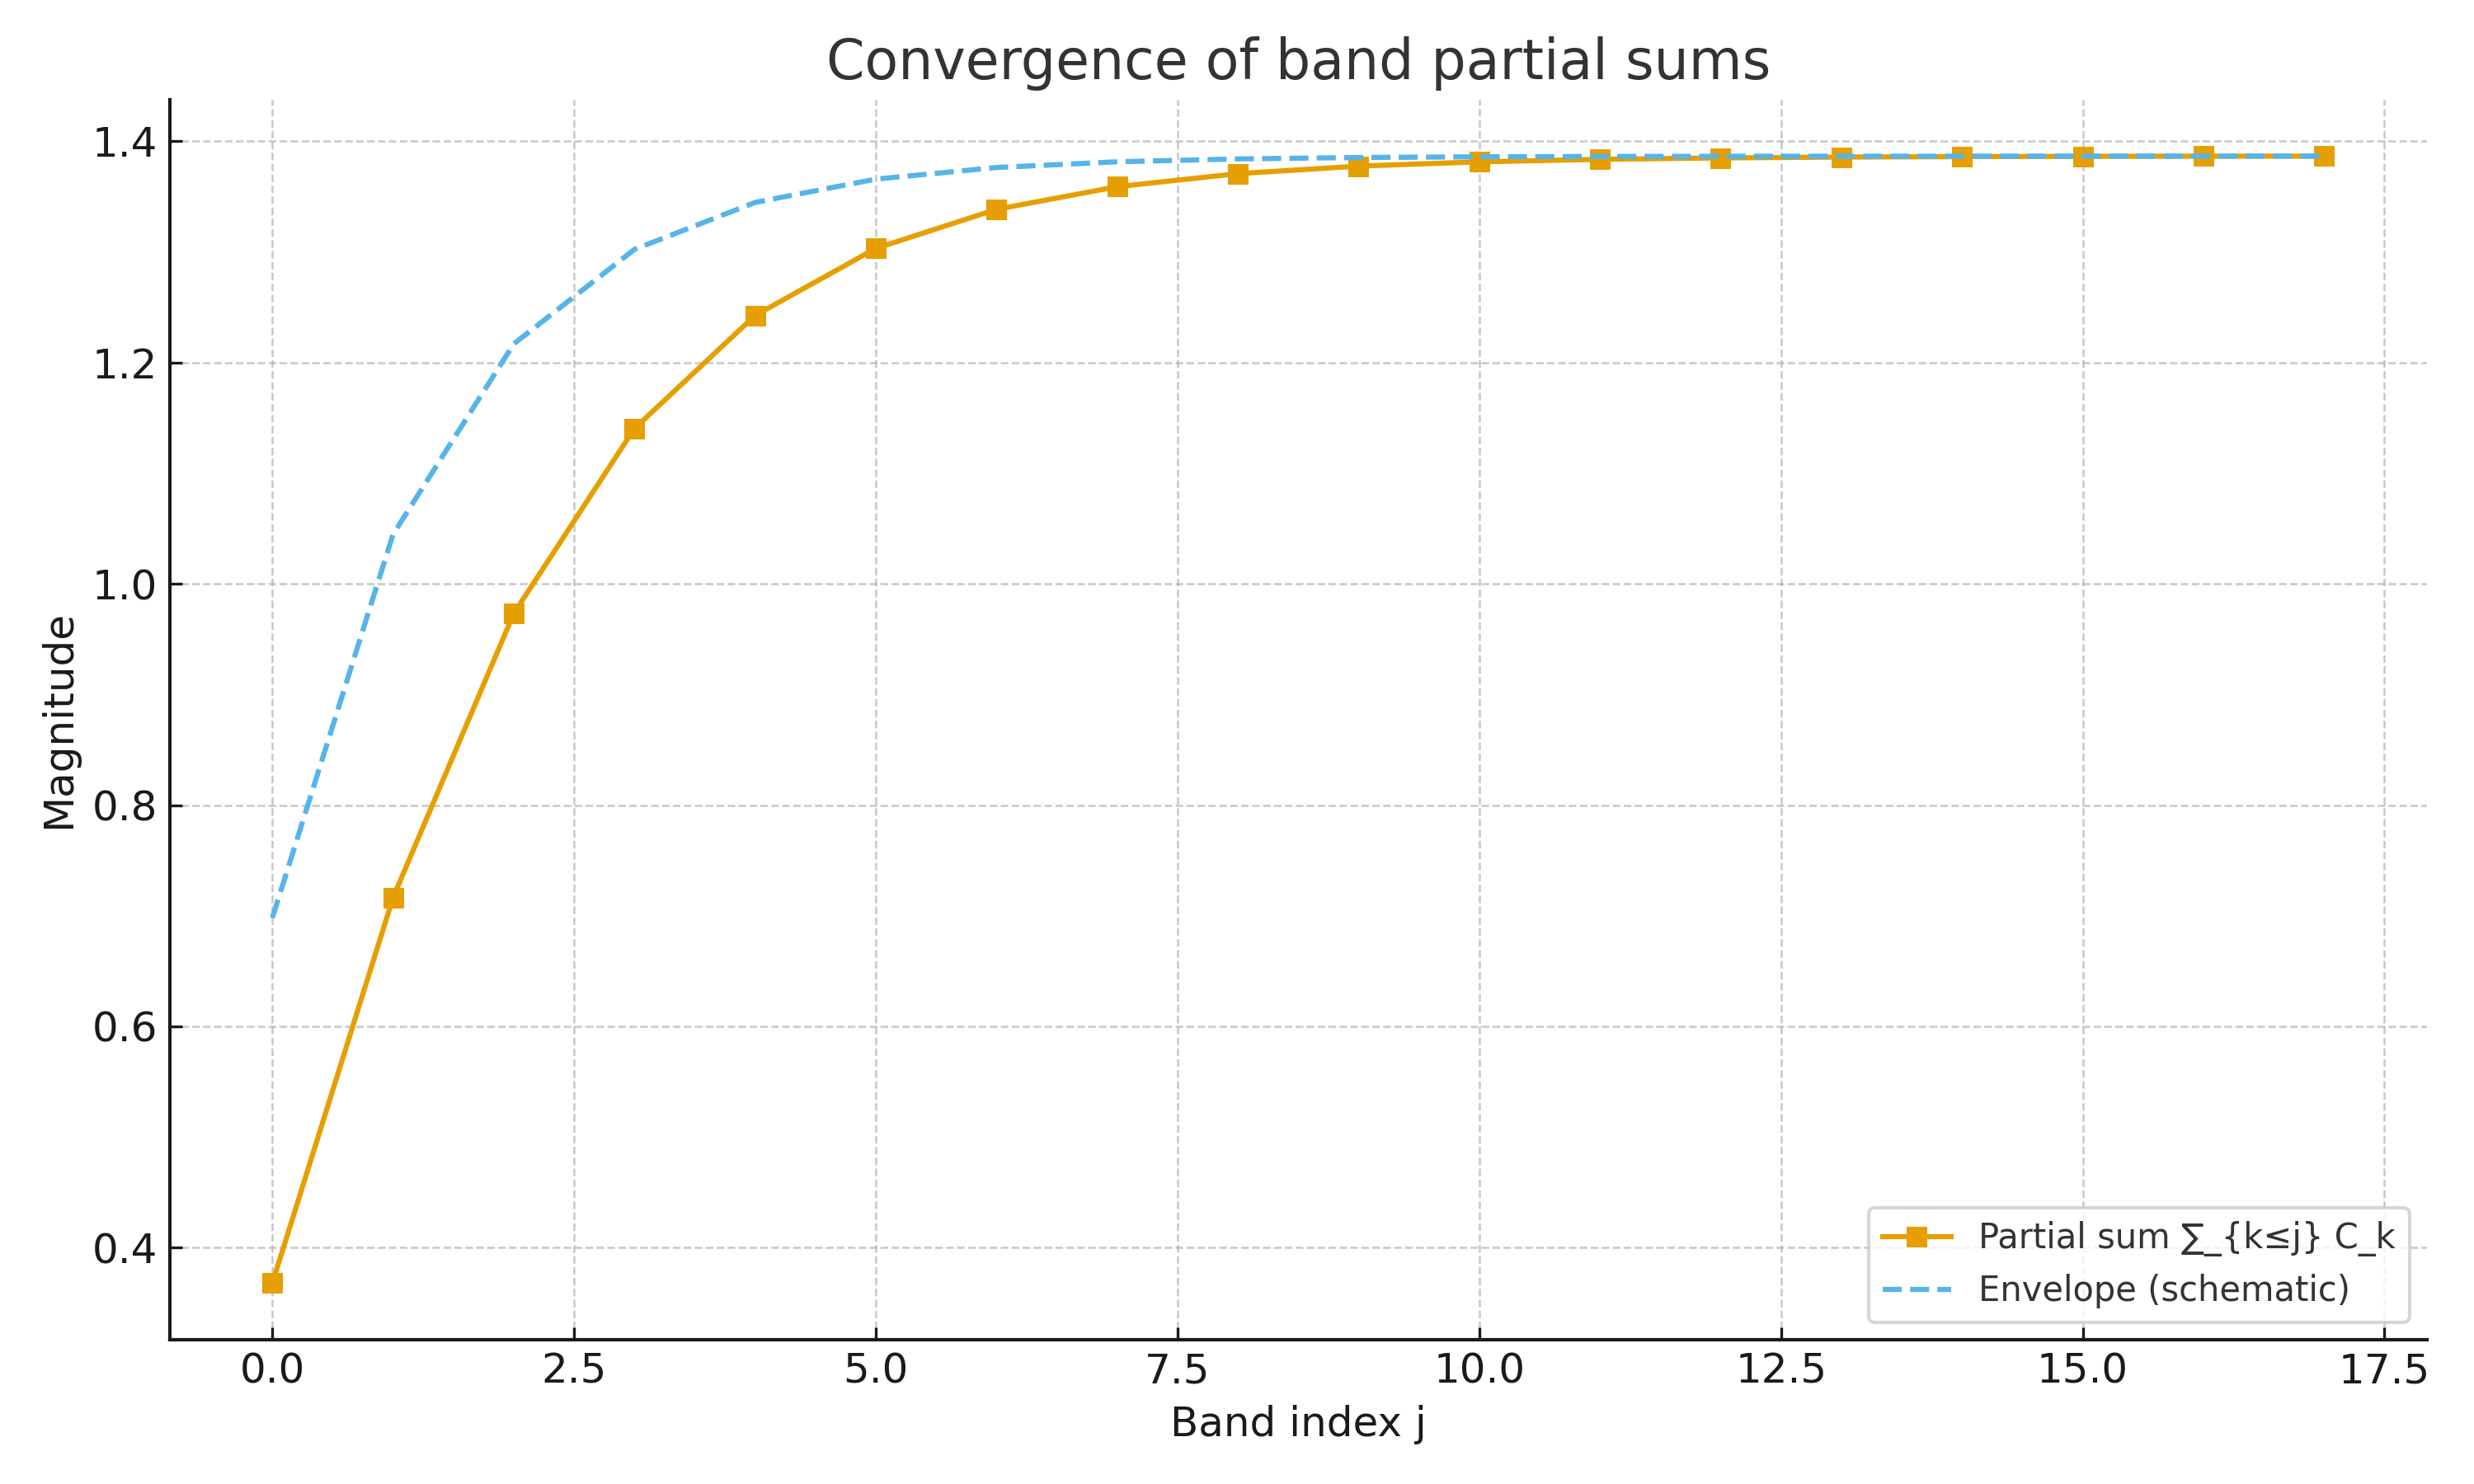
\includegraphics[width=0.75\linewidth]{figures/band_partial_sums.png}
\caption{Convergence of partial sums $\sum_{k\le j} C_k$ (schematic).}
\end{figure}

\begin{figure}[h]
\centering
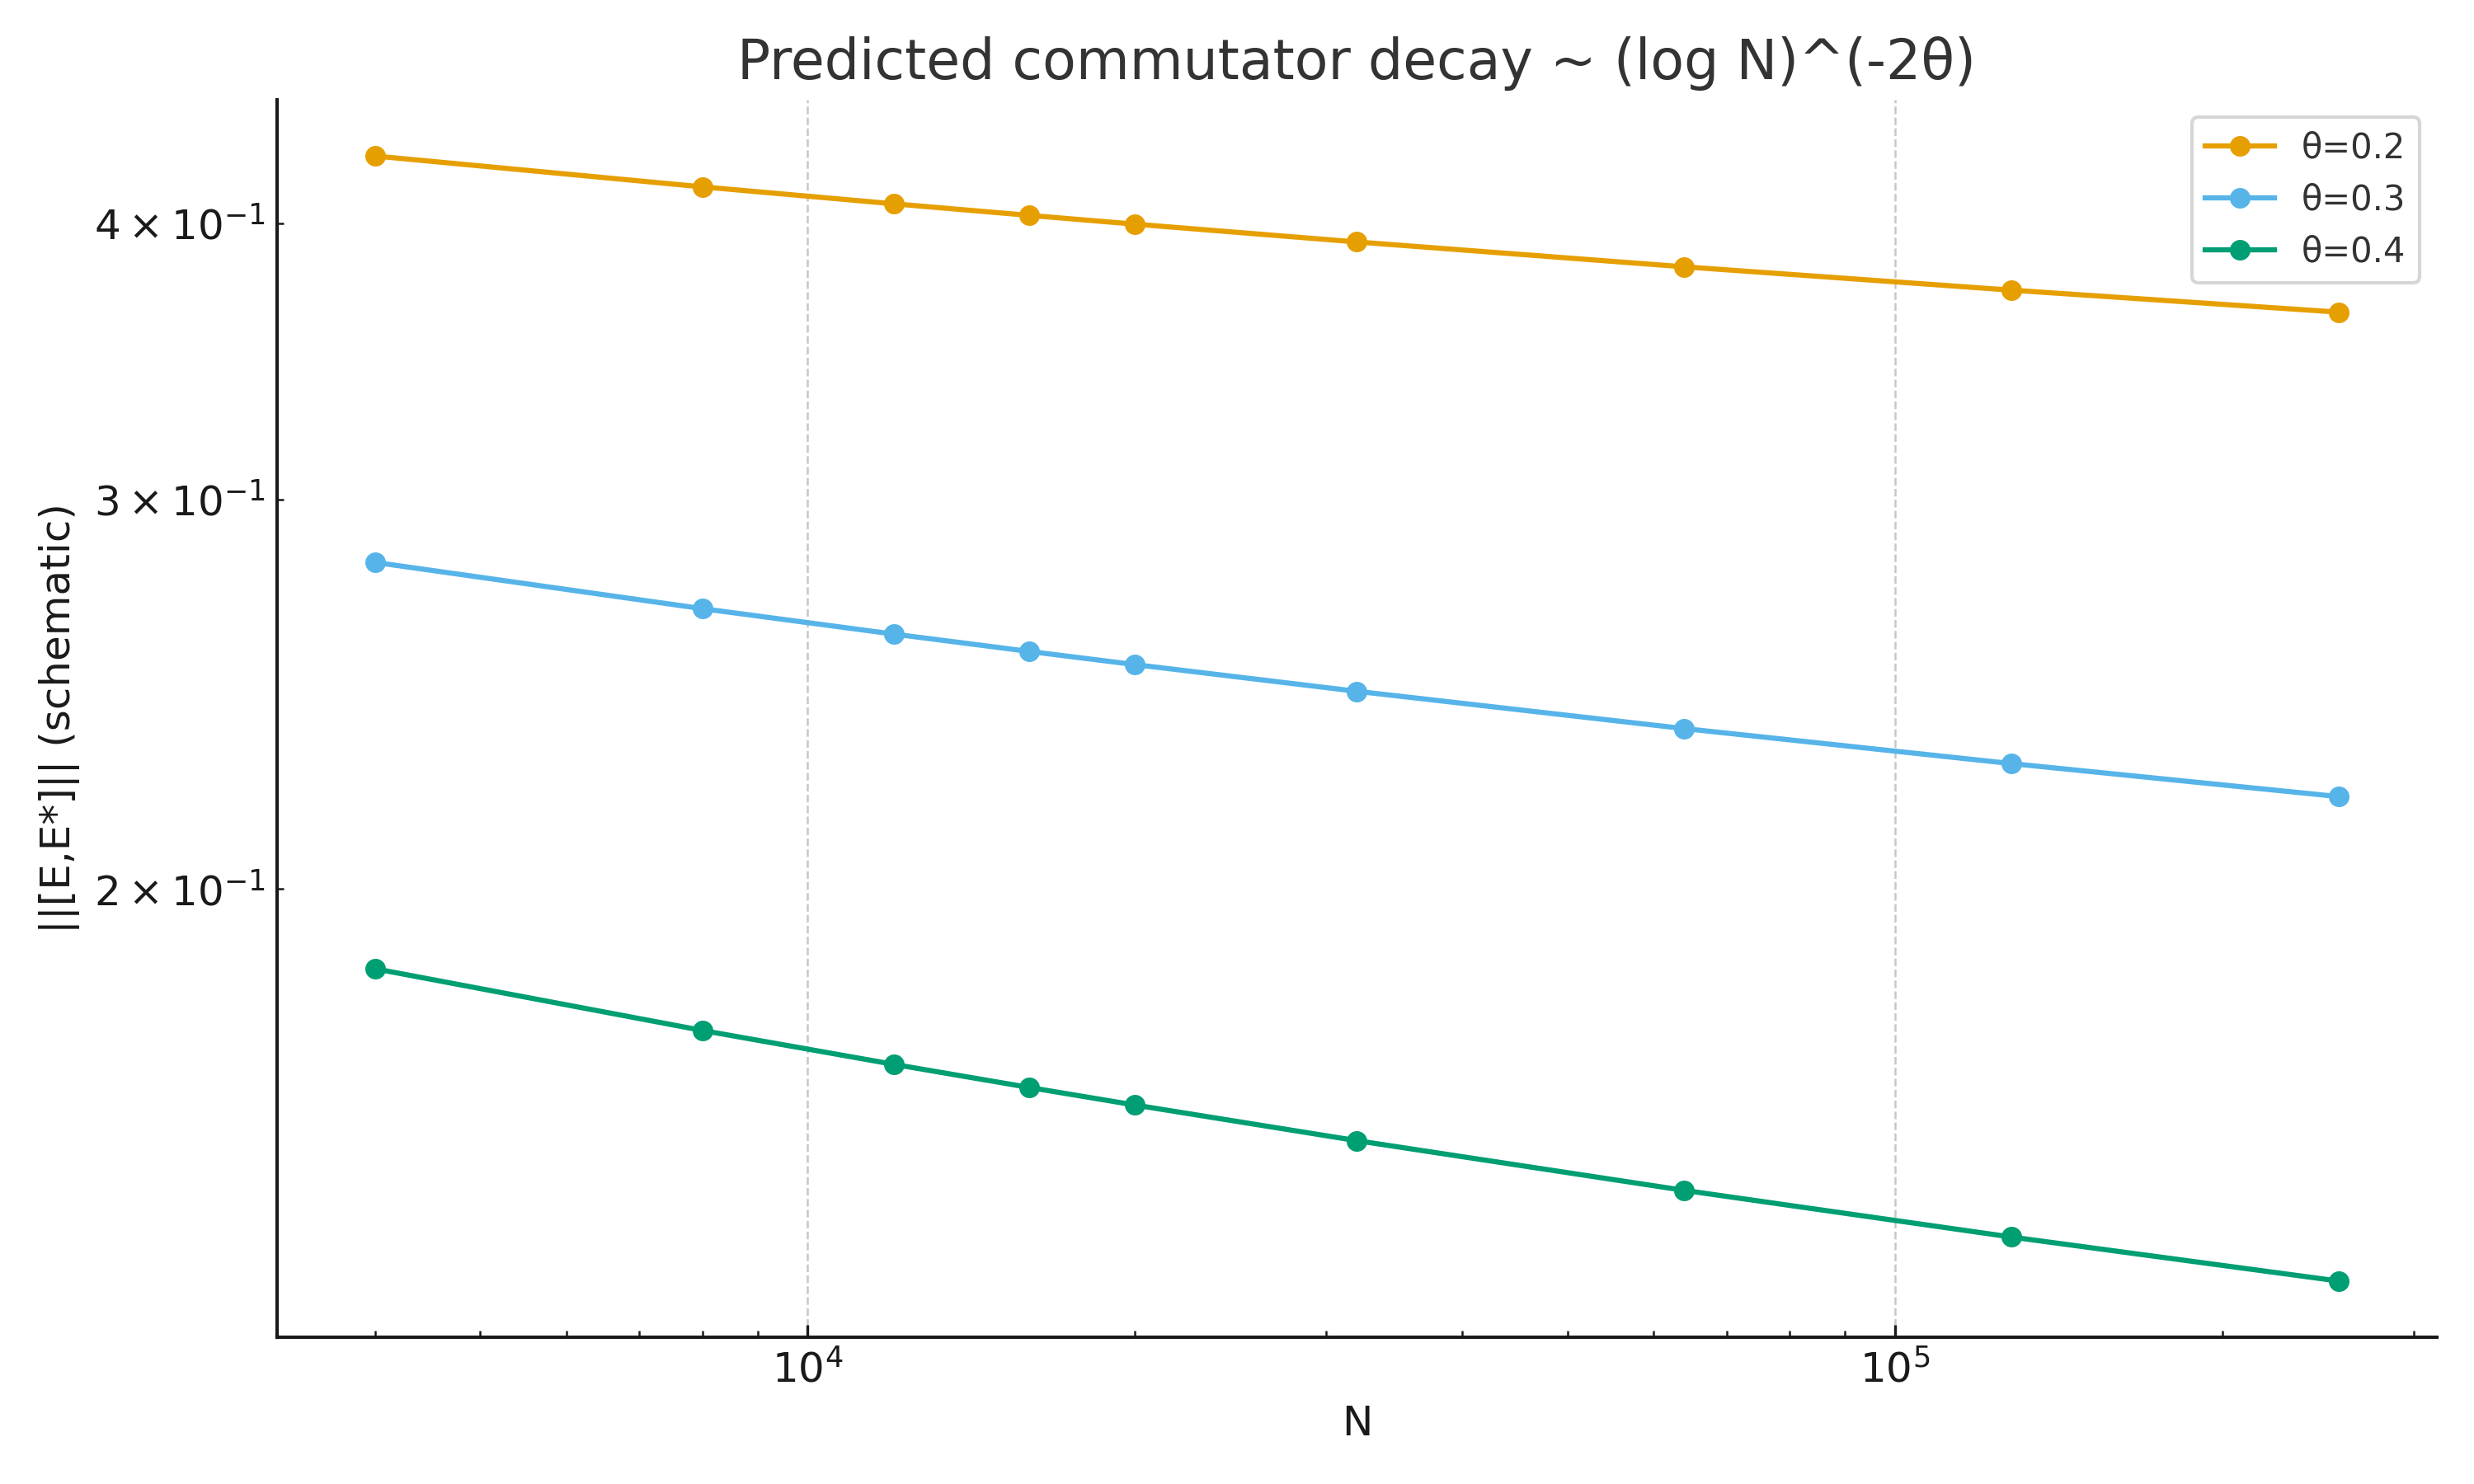
\includegraphics[width=0.75\linewidth]{figures/commutator_decay_multi.png}
\caption{Near-normality: predicted decay $\|[E,E^\ast]\|\sim (\log N)^{-2\theta}$.}
\end{figure}

\section*{Notes and Limits}
This note isolates a robust piece of the NB/BD machinery.
It does not address the full analytic continuation and zero-free region refinements
that would be required to imply RH. The aim is to present a portable lemma with
transparent constants and explicit $\varepsilon$--$\theta$ tracking.

\end{document}
